\documentclass{standalone}
\usepackage{tikz}
\usetikzlibrary{patterns, positioning}
\usepackage[sfdefault]{ClearSans} %% option 'sfdefault' activates Clear Sans as the default text font
\usepackage[T1]{fontenc}

\begin{document}
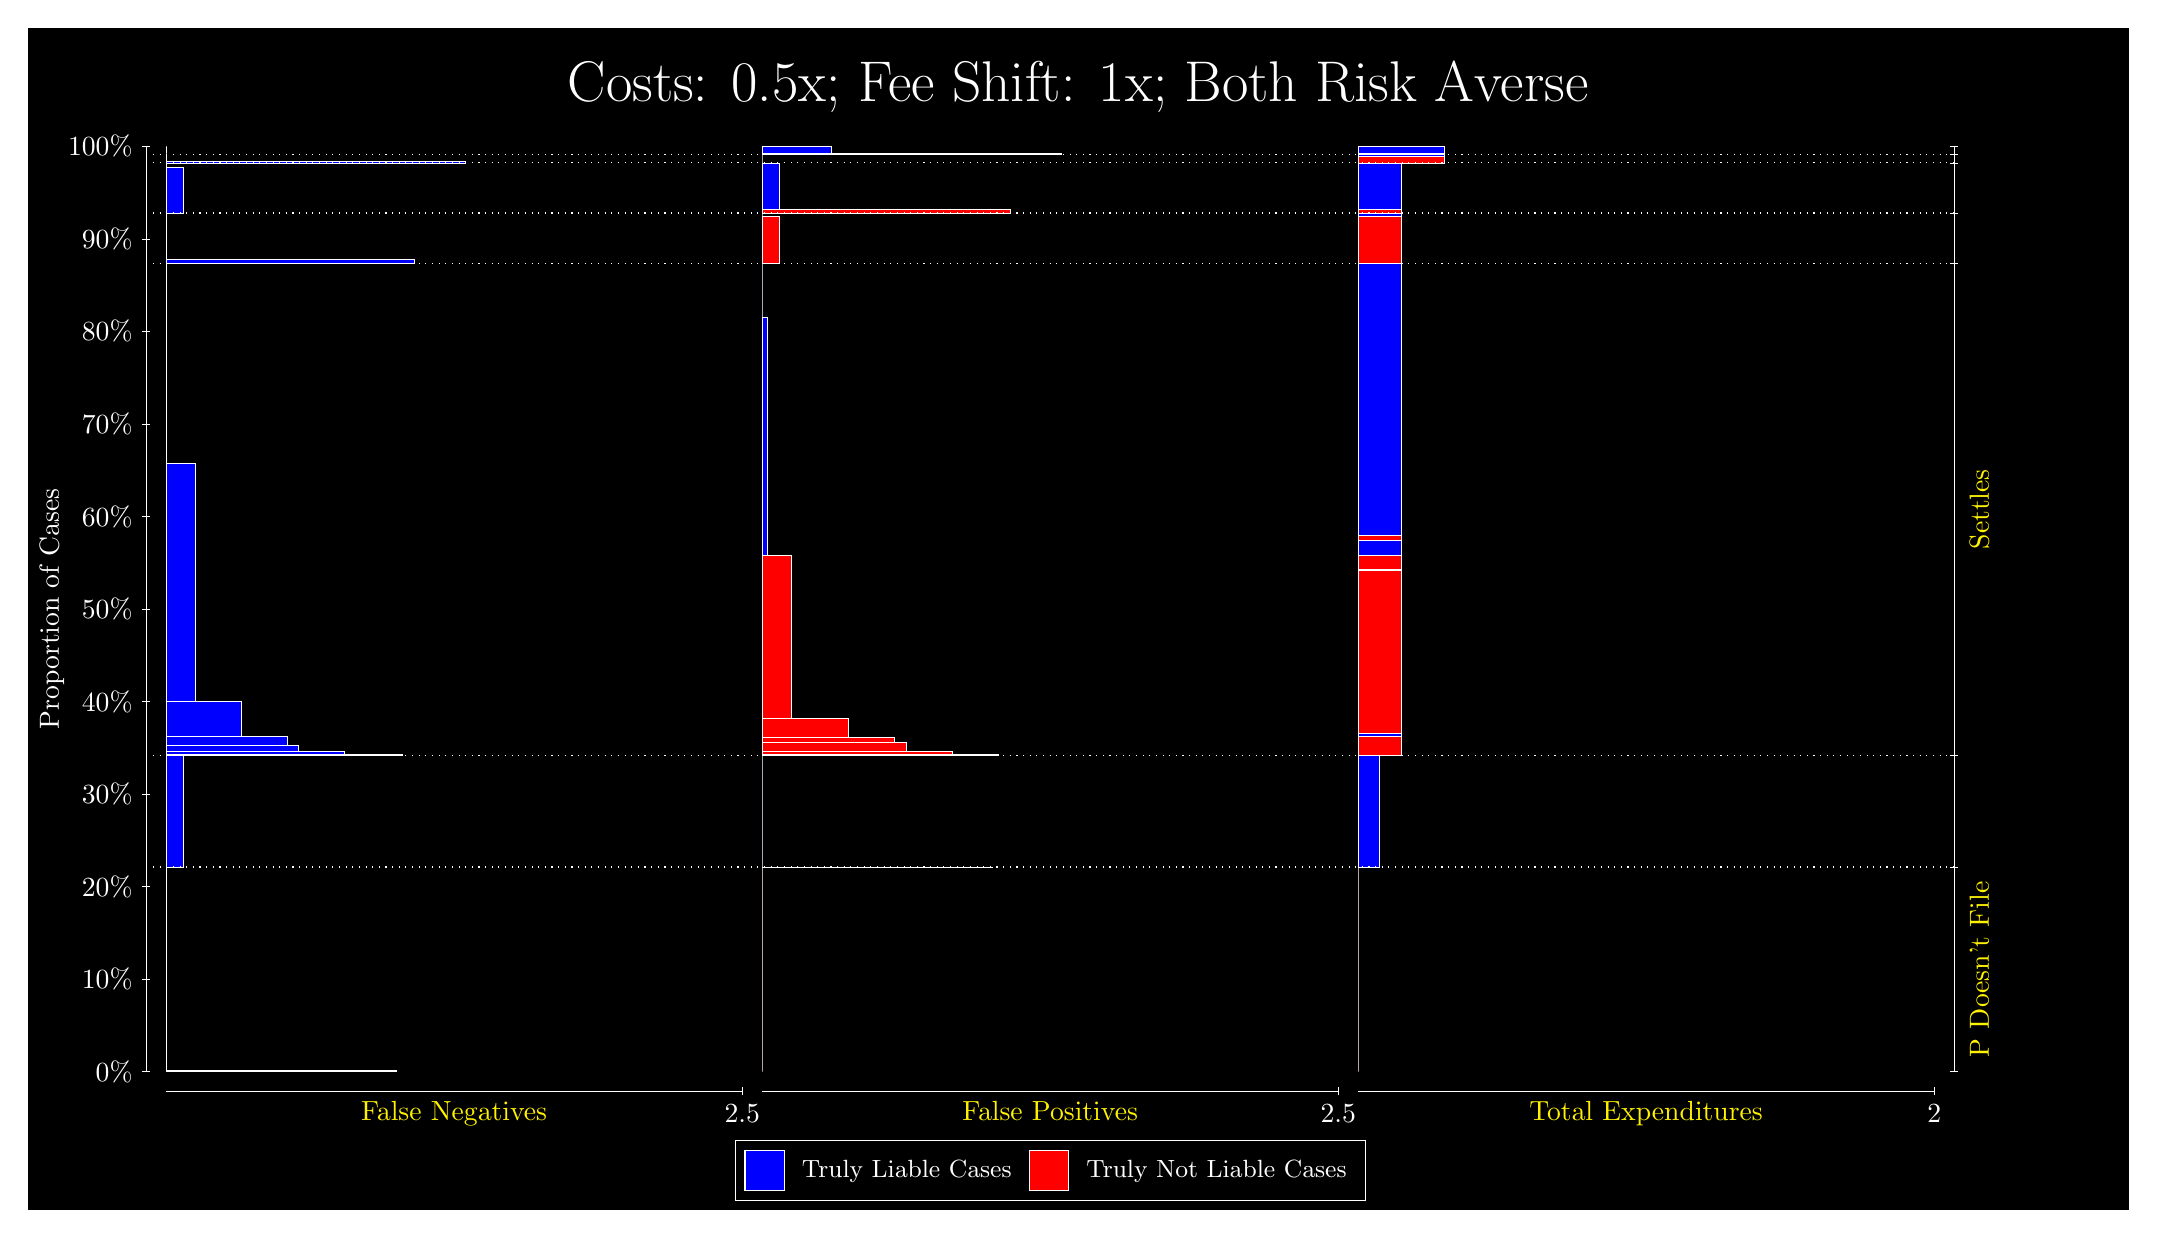
\begin{tikzpicture}
\draw[fill=black] (0,0) rectangle (26.667,15);
\draw[text=white] (0,13.5) rectangle (26.667,15) node[midway] {\huge Costs: 0.5x; Fee Shift: 1x; Both Risk Averse};
\draw[white, very thin] (1.5,1.75) -- (1.5,13.5);
\node[rotate=90, text=white, anchor=center] at (0.3, 7.625) {Proportion of Cases};
\draw[white, very thin] (1.45,1.75) -- (1.55,1.75);
\node[text=white, anchor=east] at (1.45, 1.75) {0\%};
\draw[white, very thin] (1.45,2.925) -- (1.55,2.925);
\node[text=white, anchor=east] at (1.45, 2.925) {10\%};
\draw[white, very thin] (1.45,4.1) -- (1.55,4.1);
\node[text=white, anchor=east] at (1.45, 4.1) {20\%};
\draw[white, very thin] (1.45,5.275) -- (1.55,5.275);
\node[text=white, anchor=east] at (1.45, 5.275) {30\%};
\draw[white, very thin] (1.45,6.45) -- (1.55,6.45);
\node[text=white, anchor=east] at (1.45, 6.45) {40\%};
\draw[white, very thin] (1.45,7.625) -- (1.55,7.625);
\node[text=white, anchor=east] at (1.45, 7.625) {50\%};
\draw[white, very thin] (1.45,8.8) -- (1.55,8.8);
\node[text=white, anchor=east] at (1.45, 8.8) {60\%};
\draw[white, very thin] (1.45,9.975) -- (1.55,9.975);
\node[text=white, anchor=east] at (1.45, 9.975) {70\%};
\draw[white, very thin] (1.45,11.15) -- (1.55,11.15);
\node[text=white, anchor=east] at (1.45, 11.15) {80\%};
\draw[white, very thin] (1.45,12.325) -- (1.55,12.325);
\node[text=white, anchor=east] at (1.45, 12.325) {90\%};
\draw[white, very thin] (1.45,13.5) -- (1.55,13.5);
\node[text=white, anchor=east] at (1.45, 13.5) {100\%};

\draw[white, very thin] (24.457,1.75) -- (24.457,13.5);
\draw[white, very thin] (24.407,1.75) -- (24.507,1.75);
\node[anchor=west] at (24.407, 1.75) {};
\draw[white, very thin] (24.407,4.3472) -- (24.507,4.3472);
\node[anchor=west] at (24.407, 4.3472) {};
\draw[white, very thin] (24.407,5.7655) -- (24.507,5.7655);
\node[anchor=west] at (24.407, 5.7655) {};
\draw[white, very thin] (24.407,12.016) -- (24.507,12.016);
\node[anchor=west] at (24.407, 12.016) {};
\draw[white, very thin] (24.407,12.653) -- (24.507,12.653);
\node[anchor=west] at (24.407, 12.653) {};
\draw[white, very thin] (24.407,13.289) -- (24.507,13.289);
\node[anchor=west] at (24.407, 13.289) {};
\draw[white, very thin] (24.407,13.395) -- (24.507,13.395);
\node[anchor=west] at (24.407, 13.395) {};
\draw[white, very thin] (24.407,13.5) -- (24.507,13.5);
\node[anchor=west] at (24.407, 13.5) {};

\draw[white, very thin, fill=blue] (1.75,1.75) rectangle (4.6775,1.7637);
\draw[white, very thin, fill=red] (1.75,1.7637) rectangle (1.75,4.3472);
\draw[white, very thin, fill=blue] (1.75,4.3472) rectangle (1.9696,5.7625);
\draw[white, very thin, fill=red] (1.75,5.7625) rectangle (1.75,5.7655);
\draw[white, very thin, fill=blue] (1.75,5.7655) rectangle (4.7507,5.7844);
\draw[white, very thin, fill=blue] (1.75,5.7844) rectangle (4.0188,5.8153);
\draw[white, very thin, fill=blue] (1.75,5.8153) rectangle (3.4333,5.8942);
\draw[white, very thin, fill=blue] (1.75,5.8942) rectangle (3.287,6.0132);
\draw[white, very thin, fill=blue] (1.75,6.0132) rectangle (2.7015,6.4517);
\draw[white, very thin, fill=blue] (1.75,6.4517) rectangle (2.1159,9.4752);
\draw[white, very thin, fill=red] (1.75,9.4752) rectangle (1.75,12.016);
\draw[white, very thin, fill=blue] (1.75,12.016) rectangle (4.8971,12.063);
\draw[white, very thin, fill=red] (1.75,12.063) rectangle (1.75,12.653);
\draw[white, very thin, fill=blue] (1.75,12.653) rectangle (1.9696,13.238);
\draw[white, very thin, fill=red] (1.75,13.238) rectangle (1.75,13.289);
\draw[white, very thin, fill=blue] (1.75,13.289) rectangle (5.5558,13.306);
\draw[white, very thin, fill=red] (1.75,13.306) rectangle (1.75,13.395);
\draw[white, very thin, fill=red] (1.75,13.395) rectangle (1.75,13.411);
\draw[white, very thin, fill=blue] (1.75,13.411) rectangle (1.75,13.5);
\draw[white, very thin, fill=red] (9.3189,1.75) rectangle (9.3189,4.3335);
\draw[white, very thin, fill=blue] (9.3189,4.3335) rectangle (9.3189,4.3472);
\draw[white, very thin, fill=red] (9.3189,4.3472) rectangle (12.246,4.3503);
\draw[white, very thin, fill=blue] (9.3189,4.3503) rectangle (9.3189,5.7655);
\draw[white, very thin, fill=red] (9.3189,5.7655) rectangle (12.32,5.7819);
\draw[white, very thin, fill=red] (9.3189,5.7819) rectangle (11.734,5.8198);
\draw[white, very thin, fill=red] (9.3189,5.8198) rectangle (11.149,5.9283);
\draw[white, very thin, fill=red] (9.3189,5.9283) rectangle (11.002,5.9908);
\draw[white, very thin, fill=red] (9.3189,5.9908) rectangle (10.417,6.2392);
\draw[white, very thin, fill=red] (9.3189,6.2392) rectangle (9.6848,8.3068);
\draw[white, very thin, fill=blue] (9.3189,8.3068) rectangle (9.3921,11.33);
\draw[white, very thin, fill=blue] (9.3189,11.33) rectangle (9.3189,12.016);
\draw[white, very thin, fill=red] (9.3189,12.016) rectangle (9.5384,12.606);
\draw[white, very thin, fill=blue] (9.3189,12.606) rectangle (9.3189,12.653);
\draw[white, very thin, fill=red] (9.3189,12.653) rectangle (12.466,12.705);
\draw[white, very thin, fill=blue] (9.3189,12.705) rectangle (9.5384,13.289);
\draw[white, very thin, fill=red] (9.3189,13.289) rectangle (9.3189,13.378);
\draw[white, very thin, fill=blue] (9.3189,13.378) rectangle (9.3189,13.395);
\draw[white, very thin, fill=red] (9.3189,13.395) rectangle (13.125,13.411);
\draw[white, very thin, fill=blue] (9.3189,13.411) rectangle (10.197,13.5);
\draw[white, very thin, fill=red] (16.888,1.75) rectangle (16.888,4.3335);
\draw[white, very thin, fill=blue] (16.888,4.3335) rectangle (16.888,4.3472);
\draw[white, very thin, fill=red] (16.888,4.3472) rectangle (17.162,4.3503);
\draw[white, very thin, fill=blue] (16.888,4.3503) rectangle (17.162,5.7655);
\draw[white, very thin, fill=red] (16.888,5.7655) rectangle (17.437,6.0139);
\draw[white, very thin, fill=blue] (16.888,6.0139) rectangle (17.437,6.0448);
\draw[white, very thin, fill=red] (16.888,6.0448) rectangle (17.437,8.1123);
\draw[white, very thin, fill=blue] (16.888,8.1123) rectangle (17.437,8.1312);
\draw[white, very thin, fill=red] (16.888,8.1312) rectangle (17.437,8.3022);
\draw[white, very thin, fill=blue] (16.888,8.3022) rectangle (17.437,8.5002);
\draw[white, very thin, fill=red] (16.888,8.5002) rectangle (17.437,8.5545);
\draw[white, very thin, fill=blue] (16.888,8.5545) rectangle (17.437,12.016);
\draw[white, very thin, fill=red] (16.888,12.016) rectangle (17.437,12.606);
\draw[white, very thin, fill=blue] (16.888,12.606) rectangle (17.437,12.653);
\draw[white, very thin, fill=red] (16.888,12.653) rectangle (17.437,12.705);
\draw[white, very thin, fill=blue] (16.888,12.705) rectangle (17.437,13.289);
\draw[white, very thin, fill=red] (16.888,13.289) rectangle (17.986,13.378);
\draw[white, very thin, fill=blue] (16.888,13.378) rectangle (17.986,13.395);
\draw[white, very thin, fill=red] (16.888,13.395) rectangle (17.986,13.411);
\draw[white, very thin, fill=blue] (16.888,13.411) rectangle (17.986,13.5);
\draw[white, dotted] (1.5,4.3472) -- (24.457,4.3472);
\draw[white, dotted] (1.5,5.7655) -- (24.457,5.7655);
\draw[white, dotted] (1.5,12.016) -- (24.457,12.016);
\draw[white, dotted] (1.5,12.653) -- (24.457,12.653);
\draw[white, dotted] (1.5,13.289) -- (24.457,13.289);
\draw[white, dotted] (1.5,13.395) -- (24.457,13.395);
\draw[white, very thin] (1.75,1.5) -- (9.0689,1.5);
\node[text=yellow, anchor=north] at (5.4094, 1.5) {False Negatives};
\draw[white, very thin] (9.0689,1.45) -- (9.0689,1.55);
\node[text=white, anchor=north] at (9.0689, 1.45) {2.5};

\draw[white, very thin] (9.3189,1.5) -- (16.638,1.5);
\node[text=yellow, anchor=north] at (12.978, 1.5) {False Positives};
\draw[white, very thin] (16.638,1.45) -- (16.638,1.55);
\node[text=white, anchor=north] at (16.638, 1.45) {2.5};

\draw[white, very thin] (16.888,1.5) -- (24.207,1.5);
\node[text=yellow, anchor=north] at (20.547, 1.5) {Total Expenditures};
\draw[white, very thin] (24.207,1.45) -- (24.207,1.55);
\node[text=white, anchor=north] at (24.207, 1.45) {2};

\node[text=yellow, centered, rotate=90] at (24.777, 3.0486) {P Doesn't File};

\node[text=yellow, centered, rotate=90] at (24.777, 8.891) {Settles};





\draw (12.978300999999998,1.5) node[draw=none] (baseCoordinate) {};
\begin{scope}[align=center]
        \matrix[scale=0.5, draw=white, below=0.5cm of baseCoordinate, nodes={draw}, column sep=0.1cm]{
            \node[rectangle, draw, minimum width=0.5cm, minimum height=0.5cm, fill=blue] {}; &
            \node[draw=none, font=\small, text=white] (B) {Truly Liable Cases}; &
            \node[rectangle, draw, minimum width=0.5cm, minimum height=0.5cm, fill=red] {}; &
            \node[draw=none, font=\small, text=white] (B) {Truly Not Liable Cases}; \\
            };
\end{scope}

\end{tikzpicture}
\end{document}